\documentclass[10pt]{amsart} 
\usepackage{graphicx} 
\usepackage{float} % necessary for placement of figures
\usepackage{amsmath}
\usepackage{tabularx}
\usepackage{gensymb}
\usepackage[style = authoryear, sorting = nyt, backend = biber]{biblatex}
\bibliography{library.bib}

\begin{document}
\section{Managing the Department of Defense portfolio}
The Department of Defense (DoD) has defense installations and deployed assets throughout the world, in a variety of different operating environments with the mission of protecting national resources.
The DoD manages a portfolio of more than 3 million employees, several hundred thousand buildings and structures spread over more than 5,000 sites on over 30 million acres of land \parencite{dodassets2016}.
The challenges of managing these resources are immense.
From managing prescribed burning activities at Fort Bragg in North Carolina to maintain habitat for the Red Cockaded Woodpecker, as well as reduce fire danger from training activities; to the siting of a new cyber-security building at the United States Naval Academy; to ensuring the safety of air craft and personnel in the face of coastal storms at Langley Air Force Base in Hampton, VA, the challenges are varied.

\section{What is climate change?}
We know with high certainty that the earth's climate is changing largely as a result of human activity (i.e., anthropogenic emissions), which poses challenges and risks for both human and natural systems.
In the years following the Industrial Revolution the concentration of $CO_2$ and other greenhouse gases in the atmosphere has been increasing, largely as a result of emissions from human activity.
While $CO_2$ and other greenhouse gases have always been present in the atmosphere they haven't been found at present day concentrations over any period during the past 400,000 years, as shown by repeated study of ice core data \parencite{}[insert citation].

$CO_2$ traps heat and warms the atmosphere, a process which makes the planet habitable, and is often referred to as the greenhouse effect. 
The greenhouse effect is a natural warming process in which solar radiation is absorbed by radiatively active gases in the atmosphere (i.e., greenhouse gases), which then radiate the energy in all directions.
Part of this energy is directed towards the surface, which results in warming with the strength of the warming depending upon the temperature of the atmosphere, as well as the amount of greenhouse gases in the atmosphere.
Since preindustrial times the amount of $CO_2$ in the atmosphere has increased by approximately 40\%.
As we have continued to emit greenhouse gases into the atmosphere we have intensified the natural greenhouse effect, which has resulted in changes to global, regional, and local temperature and precipitation patterns.

\section{Climate change: what are the uncertainties?}
The Intergovernmental Panel on Climate Change (IPCC) was created by the United Nations Environment Program (UNEP) in order to "provide the world with a clear scientific view on the current state of knowledge in climate change and its potential environmnetal and socio-economic impacts" \parencite[1]{ipcc2016organization}. 
Every few years the IPCC synthesizes the present state of climate change research into Assessment reports.
Increasingly, the reports are focusing on the information needs of stakeholders and decision makers who are attempting to determine climate change impacts, as well as adaptation alternatives.
Furthermore, the IPCC is adjusting its language to better reflect the needs of this disparate user community to ensure the proper communication of certainty around individual research results.

The scientific community is increasingly aware of the importance of uncertainty and risk from the climate system to policy choices by decision makers.
The IPCC now includes with its findings a discussion of the degree of certainty, confidence levels, and the likelihood.
The degree of certainty in each key finding addresses the type, amount, quality, and consistency of evidence and degree of agreement across the literature \parencite[6]{ipcc2016organization}.
The levels of certainty are broken into two components: summary of the evidence, which can be limited, medium or robust, and the degree of agreement, which is low, medium or high \parencite[6]{ipcc2016organization}.
Confidence in the validity of the finding is meant to synthesize both the evaluation of evidence and agreement and can be one of five levels: very low, low, medium, high, and very high \parencite[6]{ipcc2016organization}. 
Finally, the likelihood assesses the probability of some event having occurred or likely to occur in the future \parencite[6]{ipcc2016organization}.
For example, the Fifth Assessment Report states that the risk from extreme weather events (e.g., heat waves, extreme precipitation, etc.)  
are already moderate (high confidence) and high with a 1\degree C additional warming (medium confidence) \parencite[6]{ipcc2016organization}.

However, as has been discussed in the literature and more generally in news media, there are significant sources of uncertainty in modeling climate change.
The IPCC defines uncertainty as a "cognitive state of incomplete knowledge that results from a lack of information and/or from disagreement about what is known or even knowable" \parencite{kunreuther2014integrated}.
There are uncertainties in the choice of how to parameterize global climate models, as well as significant in projecting future human behavior, all of which impact the evaluation of climate policy decisions.

The IPCC groups these uncertainties into five broad groupings: climate responses to greenhouse gas emissions and their associated impacts \footnote{[Insert some of the key climate uncertainties]}; stocks and flows of carbon and other greenhouse gases \footnote{Large uncertainties exist in regards to historical and present greenhouse gas sources and sinks for a number of economic sectors [is land use considered an economic sector? if not make explicit here] \parencite{kunreuther2014integrated}. These gaps make it more difficult to project how changes in greenhouse gases will effect the flow of GHGs in the system (and their subsequent impacts) \parencite{kunreuther2014integrated}.}; technological systems \footnote{Changes in technology is likely to be a significant driver of future greenhouse gas emissions. The deployment of these technologies will depend on their competitivness, learning behaviours, public acceptance, etc. \parencite{kunreuther2014integrated}.}; market behavior and regulatory actions \footnote{Expectations of the future and public policy through devices like policy incentives help to drive firms behavior. By there very nature these factors are uncertain \parencite{kunreuther2014integrated}.}; and, individual and firm perceptions \parencite{kunreuther2014integrated}\footnote{Risk and uncertainty perception are inherently determined at the individual and firm level with the macroeconomic impact being the accumulation of decisions made by these economic actors. The behavior of these groups is uncertain given that we can't always know their preferences or perceptions of these uncertain factors.}.
The important takeaway from this discussion is that climate models produce useful information for decision making processes.
However, it is important to account for these uncertainties and the sensitivity of results to them while considering impacts and adaptation alternatives. 

[Insert more of a discussion on the uncertainties and why they matter]

\section{Climate change: Why vulnerability analyses?}
Climate change is causing observable changes to human and natural systems throughout the world.
For many regions, climate change is altering hydrological systems, which then affects both the quantity and quality of water resources for the region \parencite{field2014summary}.
Species are increasingly adapting their behavior to the changing climate (i.e., altered geographic ranges, timing of activities, migration patterns, etc.) \parencite{field2014summary}.
Negative health impacts are changing as changes to temperature and rainfall patterns alter the location and prevalence of disease vectors and waterborne illnesses \parencite{field2014summary}.
Climate hazards exacerbate preexisting stressors especially for those most vulnerable \parencite{field2014summary}.
Research suggests a relationship between violent conflict and vulnerability to climate change \parencite{field2014summary}.
Finally, recent extreme climate events suggest that existing human and natural systems are highly vulnerable to current climate vulnerability (let alone future vulnerability) \parencite{field2014summary}.

\begin{figure}[H]\label{fig:impacts}
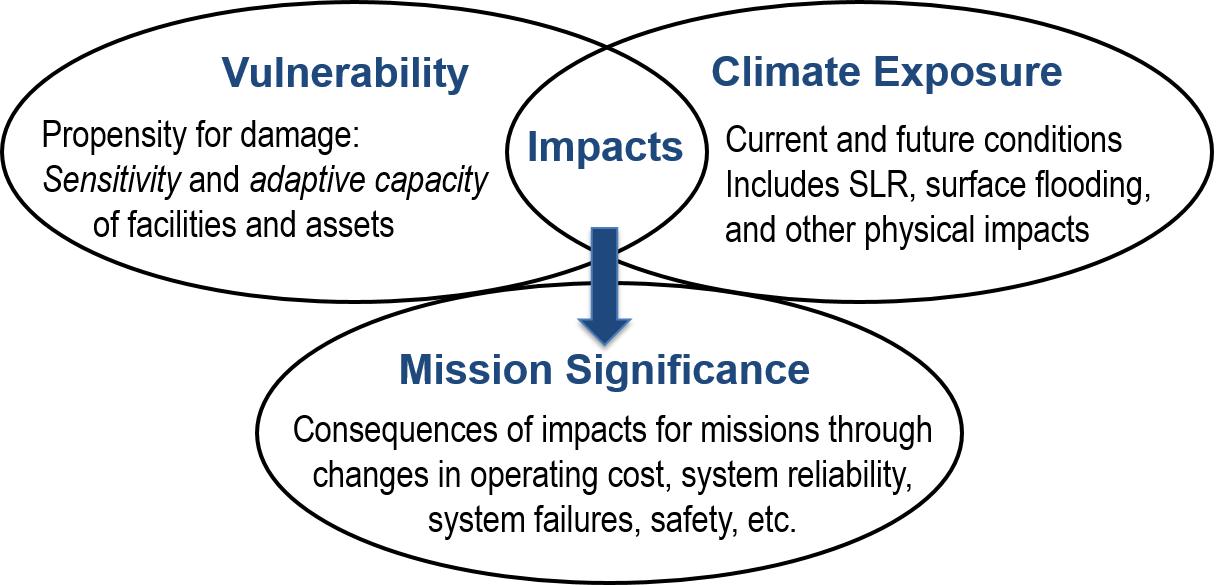
\includegraphics[width=12cm]{impacts.png}
\caption{Test}
\end{figure}

An important consideration is that human systems currently deployed around the world were mostly designed for a stationary environment that is well characterized by the information available at the time of their construction.
Climate change is a non-stationary process, which means that the environmental conditions faced by infrastructure are apt to change across the lifetime of the structure. 
For infrastructure in particular this means that at some point in the near to long-term future we could exceed the design parameters with some non-zero probability.
Climate change will continue to effect the ability of the military to meet its training objectives; impact the siting of future infrastructure; affect the costs of maintaining and operating present infrastructure, and the deployment of personnel and assets for future needs.
The ability of these installations to meet training and mission objectives depends on the consideration and incorporation of climate change effects into existing decision making and planning practices. 

\begin{tabular}{ |p{2.5cm}|p{2.5cm}|p{2.5cm}|p{2.5cm}|p{2.5cm}| }
\hline
\multicolumn{5}{|c|}{Impacts and Decisions} \\
\hline
Exposure & Impacts & Significance & Risk Management & Climate information inputs \\
\hline
Increased fire risk & Fewer burn days; ecosystem management; RCW & Costs; restrictions on ranges & Scheduling/budget; alter management; add training capacity at other installations & T, P, wind, soil moisture, fuel load \\
\hline
Ecosystem migration (change in flora/fauna ranges) & Protected species; invasive species; movement of pests; disease vectors & Costs; range suitability or availability & Alter management; redistribute training activities & Average and extremes of T, P, and other variables \\
\hline
Increase in days with extreme heat & Outdoor activity and training restrictions; energy system stress & Reduced training throughput; service interruptions & Alter training regimen; redistribute training activities & T, P, wind, solar insolation \\
\hline
Change in surface wind speed & Flight training, parachute drops; controlled burns & Training, ecosystem maintenance & Alter training regimen; redistribute training activities; change burn patterns & Daytime daily wind threshold exceedance \\
\hline
\end{tabular}

Recently, a number of Executive Orders issued to force the consideration of climate change in planning and decision processes in government agencies. 
The Department of Defense is required by Executive Order 13514 to assess its climate change risks and vulnerabilities, and to manage the effects of climate change on its operations and mission in both the near and longer term. 
Executive Order 13653 built upon Executive Order 13514 by requiring that each agency develop, implement, and update (maintain) agency climate adaptation plans.
The goal of these plans was to integrate climate considerations into existing planning, operations, and mission objectives of each agency.

Stakeholders should be concerned about the impacts of climate on their ability to do their jobs. 
But the impacts of climate change are unlikely to be evenly distributed across all personnel and assets in the DoD portfolio, which as a result requires some vulnerability screening.
The vulnerability screening process seeks to create a ranked ordering of assets, sites, or missions along a vulnerability dimension through a collaborative effort of experts and stakeholders.
The end result of the effort is an ordered list of assets that can be used for assigning the need for further vulnerability analyses. 

\section{Vulnerability assessments: A three tiered approach}
Given a need to conduct vulnerability assessment from a regulatory and risk management perspective it is still not clear how one might go about conducting one.
We know that exposure and vulnerabilities are non-homogenous across a portfolio of assets, sites or installations. 
Instead, particular sites and assets are more vulnerable than others.
Given this reality, it is economically inefficient to allocate vulnerability analysis resources evenly across the entire portfolio.
We believe that a tiered approach is capable of addressing the challenge of efficiently allocating an assessment budget.
We divide the complicated task into three distinct steps, which are accomplished over an ever decreasing set of assets: a screening, a vulnerability analysis, and adaptive planning process. 
Our approach first uses institutional datasets (i.e., property management systems, GIS data, etc.) and potentially, historical exposure data to create an indicator (i.e., a ranked ordering of all assets, sites, etc.) that determines the sites where further assessment is needed. 
In additional analyses, more and more resources are used at the site to identify particular vulnerabilities, impacts, and adaptation alternatives. 

The first tier of a vulnerability assessment screens all assets or sites to identify the set of assets or sites at higher risk to climate change such that a more detailed assessment can be undertaken at these locations.
The second tier is a site level vulnerability analysis only undertaken at those sites identified by the first tier, which delves more deeply into the particular exposure, vulnerabilities, impacts, and consequences of climate change to a particular site using a participatory process.
The Tier 2 analysis identifies whether vulnerabilities need to be addressed through additional monitoring, altered management, or structural changes.
It begins to assess the adaptation options necessary to improve resilience but these options are not yet evaluated at a level necessary for investment decisions.
Finally, a third tier assessment looks across the set of vulnerabilities identified in Tier 2 and identifies the cost effective solutions for the most pressing vulnerabilities using more detailed and costly analyses.

An example of how one might go about doing a Tier 1 assessment is through the construction of a vulnerability indicator.
In the case of the Department of Energy (DOE), we used the Facility Management System (FIMS), a real property database, to rank order program offices, by average and variance of the condition index per site in their portfolio, while simultanesouly accounting for the importance of each asset at the site. looked at the average asset conditions by site for each program office in the DOE. 
Using the average and variance we were able to construct an indicator that identified sites with poor average condition of assets or sites with a high variance in terms of the condition of assets.
The importance of the participatory process is evident in the indicator construction, as the weighting used for each asset should be a function of the importance of the asset to the mission.
Some organizations have worked to develop such metrics (i.e., mission importance index in the DOE, unique facility indicator (DOE), etc.).
But how much we should weight these assets could be developed in concert with stakeholders with the results evaluated using sensitivity analysis of the weights.



A Tier 2 analysis is developed in concert with installation personnel but produces information primarily for head quarters and major commands.
The Tier 2 assessment can be useful in establishing long-term installation led processes to improve installation resilience.
These activities might include improved data collection, maintaining databases, etc.
One challenge of this process is that it might be considered as resource extractive process from the installation.
The information collected will have a cost (i.e., increased man hours, etc.) but little direct benefit for the installation.
By this we mean that the information collected might be more useful in guiding longer temr processes, which by definition fall under the purview of headquarters processes, rather than the day-to-day functioning of the installation. 

This tension is further exacerbated by the need to engage installation managers in the process.
Participatory process (guided learning) involving owners of key systems and subject matter experts.
Require capacity building \ldots
Discussion of the participatory process role in vulnerability analyses.
Information is spread, many people have a portion of hte picture but few if any have the entire picture.
Te process leans heavily on the knowledge of both headquarters and site personnel. 
A participatory process can synthesize site-specific expertise and technical inputs needed to build resilience. 
Climate risk is a long-term process so building institutional capacity can provide some permanence to the process.


Impacts are the intersection of exposure and vulnerability.
Not all impacts have mission significance. 
Even though it hasn't been treated as such in budget processes enhancing resilience is a positive incentive.

Use of scenarios in vulnerability assessments.
The scenarios should provide a broad range of future climate conditions, acknowledging the deep uncertainty that exists in the forcing, natural variability, etc. 


The impacts of climate change on existing infrastructure are presently unknown but as a result of Executive Order [?] the military must begin the process of identifying climate vulnerabilities. 

The users of a Tier 1 assessment are likely to be headquarters or major commands.
The results of a Tier 1 assessment are meant to guide budget processes within the vulnerability assessment framework.
In that it provides input to setting priorities for vulnerability assessments at installations.




As a result, we see vulnerability analyses as part of a three tiered process. 

[insert figure]


\section{Introduction}
U.S. government agencies are now directed to assess the vulnerability of their operations and facilities to climate change and to develop adaptation plans to increase their resilience. 
Specific guidance on methods to accomplish these directives are still evolving based on the many different available frameworks. 
Our project was designed to develop and implement a vulnerability assessment framework for evaluating the vulnerability to climate change at a range of facilities in a portfolio of assets. 
This paper synthesizes lessons and insights from a series of research case studies conducted by the investigators at facilities of the U.S. Departments of Energy and Defense. 
The article elaborates on three sets of methods required to project exposure to hazards, evaluate consequences, and manage effective communications. 
In addition, suggested elements of a roadmap to support agencies in preparing for climate change, including additional methods development and capacity building, will be provided.

The literature contains a variety of proposals for conducting vulnerability assessments. 
\ldots [insert lit review]

White House steps
Step 1: Explore climate threats
Step 2: Assess vulnerability and risks
Step 3: Investigate options
Step 4: Prioritize actions
Step 5: Take action


In the next section we discuss some issues that we ran into while implementing these methods.
Next we discuss our vulnerability assessment process.
Finally, we discuss some additional takeaways from our case study experiences.

\section{Musings on existing methods}
In attempting to implement existing vulnerability methods at installations and sites in the Department of Defense and Department of Energy (DOE) portfolios we ran into several issues.

The first issue is that vulnerability analyses can have a variety of goals, outcomes, and stakeholders and there exists a tension in preventing vulnerability analyses from becoming a resource extractive effort.
By this we mean that installation managers and below often have the information necessary to determine vulnerability but this information is not often cataloged, documented, etc.
Thus, it takes time and effort on their part to put the pen to paper, fill out a new spreadsheet, sit in on presentations from academics, or be interviewed.
But the benefits of conducting a vulnerability assessment tend to be long-term and more directed towards processes of the central offices (i.e., headquarters, departments, etc.).
For example, changes in the vulnerability of an installation might feed into future siting decision making processes, which is clearly outside the purview of the installation level manager.
But it is less apparent what the benefits of conducting a vulnerability assessment are to the daily functioning of an installation in the near-term.

This is not to say that vulnerability analyses, even with their longer-term focus, cannot provide useful information to installation level managers.
For example, we found that installations tended to not know their existing vulnerabilities.
In line with existing literature people are not computers and tend to have bad memories (weighting more recent events more heavily).
Thus, it is a value added to conduct a historical assessment of vulnerabilities that they care about.
It is important to consider these types of issues given the necessary participation of these individuals in the VA process, even in non-democratic organizational structures like the military. 

We found that the participatory process is a good way to conduct these exercises \ldots
[Move participatory discussion here]

The second issue is the definition of vulnerability or a means of systematically evaluating vulnerability in a viable process.
A related issue is the need to divorce vulnerability assessments from the limitations of existing climate models.
It seems existing vulnerability assessment frameworks tend to get hung up on limits of projecting changes in exposure.
Our framework pushes forward the idea that vulnerability and exposure are independent processes and that we can push forward on one even if the other is more limited. 

Installation and facilities managers care about the consequences of climate change on their ability to meet mission (i.e., do the things they need to do).
Our vulnerability assessment framework recognizes that consequences are the result of impacts, which are the intersection of vulnerability and exposure.
By this we mean that an installation usually has a small set of vulnerabilities and the region also has a small set of exposures. 
Of these two relatively small sets there are usually only a few intersections (i.e., having both a vulnerability to a particular climate event and the climate event itself present).

The third issue we identify is that sites are often vulnerable to a small set of exposures (mentioned in the previous issue), which are often not variables generated in documents like the National Climate Assessment.
For example, Fort Bragg is highly dependent upon fire management practices to manage their training ranges. 
Any changes in the ability to conduct prescribed burning activities could lead to impacts on the ability to conduct exercises.
Therefore, the installation would like to know about changes to fire danger indices; however, these variables are not widely available at the country level let alone for the state or region.

\section{Calls for a regional approach}
The fourth issue we identify is that generating climate information outside of the data generated in processes like the National Climate Assessment is expensive.
Regional climate outlooks are one way of reducing the cost of these exercises by spreading the cost across a larger group of stakeholders.


\section{Five steps and repeat: Vulnerability assessments}
In this section we distill the results of the series of case studies we conducted to a set of steps for implementing a vulnerability analysis for an asset or site. 

\subsection{Step 1: Establish assessment team}
Goal is to define the who, what, when and how, as well as setting expectations for the process.
The team composition should include managers and technical experts related to key systems.
In the military for example, the civilian workforce is often the vessel for the corporate memory (given how much military personnel move).
The support of the installation leadership is critical in determining the outcome of hte processes. 

The internal engagement process requires careful consideration, especially for data collection.
In our case studies we tried two engagement processes.
In the first, we provided some background materials before our initial kickoff meeting, in which we brought all of the interested (and important) parties together.
The meeting was structured around providing information on climate change, climate change projections, impacts, and vulnerability assessments.
Our efforts were primarily focused on gathering buyin and identifying what data existed and who managed it. 

The alternative process involved identifying key stakeholders well in advance of the kickoff meeting.
Generating buy in and soliciting data from these individuals and coming to the initial kickoff meeting with preliminary results.
The goal of this process was to have a more informed discussion of where to go next (i.e., what do installation level managers need from us?).
However, perhaps unique to the circumstances, we identified one significant weakness with this approach; it is highly dependent upon the quality of the information.
In the particular case of Fort Bragg current documents had not been updated to reflect current conditions, which identified erosion as a major issue. 
While did not proceed as far as we might have down the erosion path, we did 'waste' some resources on this avenue.

External engagement focuses on the external dependencies.
Subject matter experts are to facilitate expert judgment and identify the SMEs for specific topics.

\subsection{Step 2: Gather information and set priorities}
Objective is to gather and synthesize existing information and identify what topics require further assessment.
Consider the upcoming decisions related to long-lived assets or future plans, not only current infrastructure/activities.
This is an iterative process that relies upon conference calls, document review, interviews, analysis and the use of extant documents and reports (i.e., INRMP, Master plans, etc.).

There are some key challenges to this step.
The identification of climate thresholds is difficult.
Attribute cancellations and damages to climate events (information capture could be improved).
Assess adaptive capacity (key elements are intangible).

\subsection{Step 3: Obtain climate information}
Goal is to understand the state of science for climate phenomena that will drive future impacts.
Distinguish information for participatory process and data for modeling.
Sources for this information include the National Climate Assessment, CLimate Resilience Toolkit.
We tested a climate change outlook approach, which is a document that assesses impacts relevant variables for facilities in the region.
It uses historical climatology to establish baselines before then assessing global climate model output for projections.
The regional coverage improves the economies of scale, as the report can be used across several installations.
We found that it was useful but resource intensive and to be really useful would require that personnel support, manage, and disseminate the report.

\subsection{Step 4: Estimate/model impacts}
Goal is to gather and synthesize information on how vulnerabilities and future conditions could interact.
Many sources and methods exist (a toolbox approach).
Extrapolations from past incidents.
Interpretation of assessements and research studies.
Statistical analysis of observations
The project budget is really going to determine the methods available.
 
\subsection{Step 5: Consider consequences and adaptations}
Objective is to evaluate the relative vulnerability and prioritize adaptation needs.
Various spreadsheet and ranking tools facilitate this step.
Importance of expert judgment of site and asset managers in considering the consequences of potential impacts.
The key questions are given potential impacts, how might missions be affected?
What next steps should be taken?
Scenario planning and other engagement methods can be useful if participants are receptive.

\subsection{Step 6: Apply, document, and learn (cycle back to Step 1)}
Do it all again!
This is a process that is always in motion.
Methods are improving, knowledge is improving, threats are emerging, etc.



\section{Conclusions}
Vulnerability assessments by their very nature are (or should be) circular.
By this we mean, stakeholders should continue to evaluate not only their vulnerabilities through the process but also the process itself.
As advancements are made in methods, models, etc. these changes should be incorporated into the process such that they are then necessarily incorporated in long-term decision making and planning activities. 
We see existing methods as getting the stakeholder to the right neighborhood (or city?), whereas future methods, models, or other advancements will get him or her to the right house. 

In complying with the requirement to conduct vulnerability assessments, include objectives of building capacity and improving resources for climate risk management.
Indicators, surveys, and stress tests can be used to systematically prioritize vulnerability assessments.
We need to consider factors such as mission criticality, condition, and location relative to exposure.
Site level vulnerability assessments can contribute to resilience.
Identify adaptation needs and build capacity for climate risk management.

Adaptation (i.e., changes in practices, infrastructure, etc.) should include improved monitoring.
Collecting better information on impacts at a site is valuable for future risk management.
Technical capacity is abundant, but more effort is required to organize it, share experience, and provide an evolving guide to resources.
Stakeholder engagement, climate information, impacts estimation and modeling, etc.



\newpage
\printbibliography
\end{document}